\documentclass{article}
\usepackage[utf8]{inputenc}

\title{Roteiro Windows Movie Maker}
\author{Pedro Augusto Duarte de Almeida}
\date{Outubro/2015}

\usepackage{natbib}
\usepackage{graphicx}

\begin{document}

\maketitle

\section{Introdução}
O Windows Movie Maker é um software (programa) de edição de vídeos da Microsoft.
Com este programa é possível que qualquer pessoa insira áudio, títulos, textos personalizados e efeitos de transição em suas fotos.

\begin{figure}[h!]
\centering
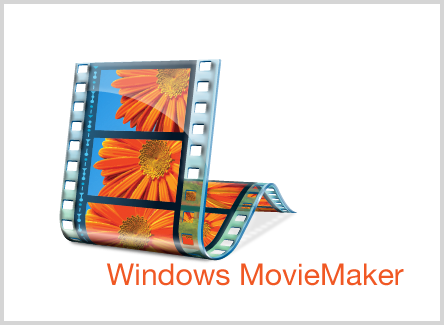
\includegraphics[scale=0.5]{movie-maker.png}
\end{figure}

Existem vários tipos de filmes que podem ser criados no Movie Maker, e um deles pode ser feito a partir de fotos tiradas com celulares, máquinas fotográficas ou filmadoras. \newline

Separe as fotos, os textos, e as músicas que pretende usar em seu filme. Uma dica importante é colocar todas as imagens imagens e músicas salvos na mesma pasta em seu computador, pois até a hora de salvar o seu projeto como filme, o Windows Movie Maker vai precisar encontrar tudo numa pasta só. Fique calmo, vamos explicar melhor ao longo do tutorial.